\section{Beschreibung der Anwendung}
\label{sec:beschreibung}
\subsection{Admindialog}
\paragraph{Wohngruppe}
Im \textit{Admindialog} können Administratoren Bewohner, Wohngruppen/-heime und Mitarbeiter verwalten.
\begin{figure*}[h]
	\begin{center}
		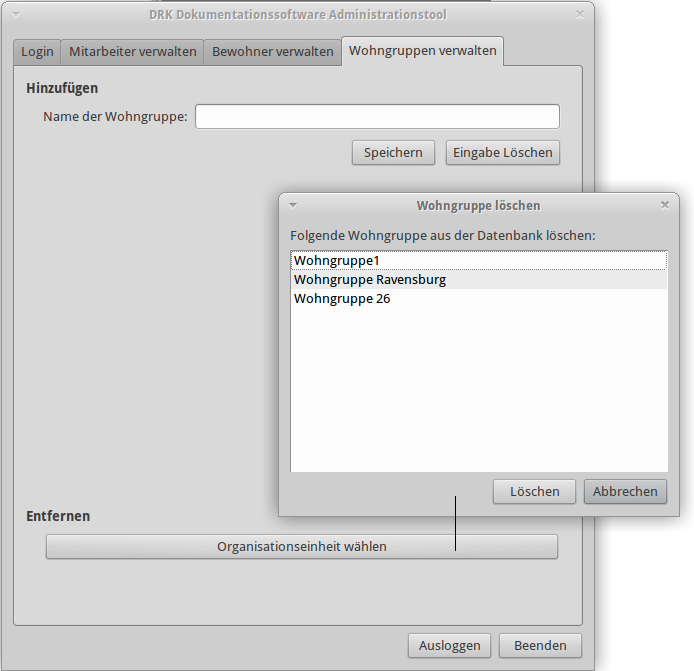
\includegraphics[keepaspectratio=true, width=0.85\textwidth]{pics/admin3.png}
		\caption{Wohngruppe}
		\label{Admindialog Wohngruppe}
		\caption{Graphen eines Interfaces}
		\label{Admindialog_Mitarbeiter_erstellen}
	\end{center}
\end{figure*}
\FloatBarrier
\noindent
Hier werden Wohngruppen erstellt, diese dienen als Gruppierung für sowohl Bewohner, als auch für Mitarbeiter.
\newpage
\noindent
\paragraph{Bewohner}
Bewohner werden mit einer Bewohnernummer, Vor-/Nachnamen und ihrer Wohngruppe  erstellt. 
\begin{figure*}[h]
	\begin{center}
		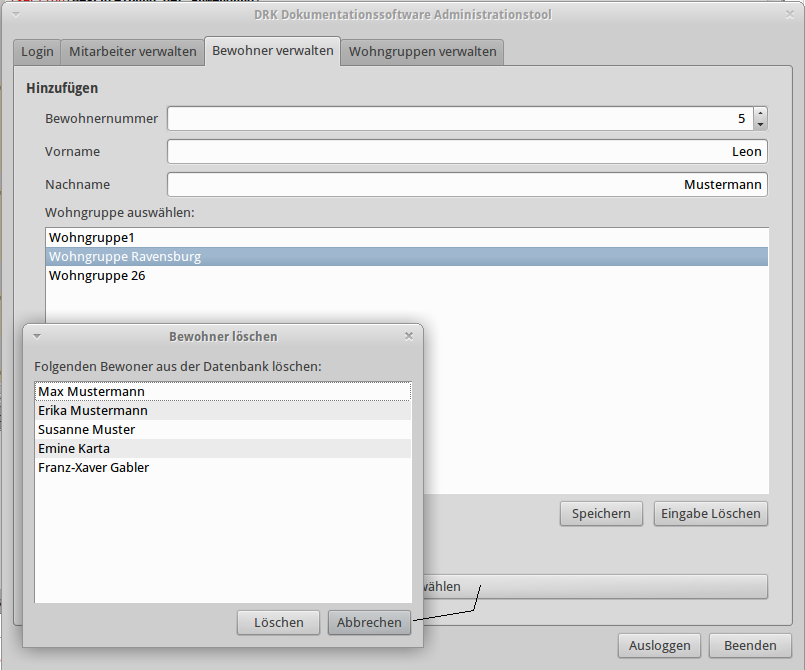
\includegraphics[keepaspectratio=true, width=0.85\textwidth]{pics/admin2.png}
		\caption{Bewohner}
		\label{Admindialog Bewohner}
		\caption{Graphen eines Interfaces}
		\label{Admindialog_Bewohner}
	\end{center}
\end{figure*}
\FloatBarrier
\noindent
Restliche Informationen werden im Client von zugewiesenen Bezugsbetreuern ausgefüllt.
\newpage
\noindent
\paragraph{Mitarbeiter}
Mitarbeiter werden mit Login sowie einigen persönlichen Daten, Name und Kontaktmöglichkeiten, sowie ihrer Berechtigung erstellt. Es ist darauf zu achten das jedem Mitarbeiter beim erstellen mindestens eine Wohngruppe zugeordnet werden muss, die er betreut. Er kann allerdings natürlich auch für mehrere Wohngruppen zuständig sein und auch der Bezugsbetreuer für Bewohner sein.
\begin{figure*}[h]
	\begin{center}
		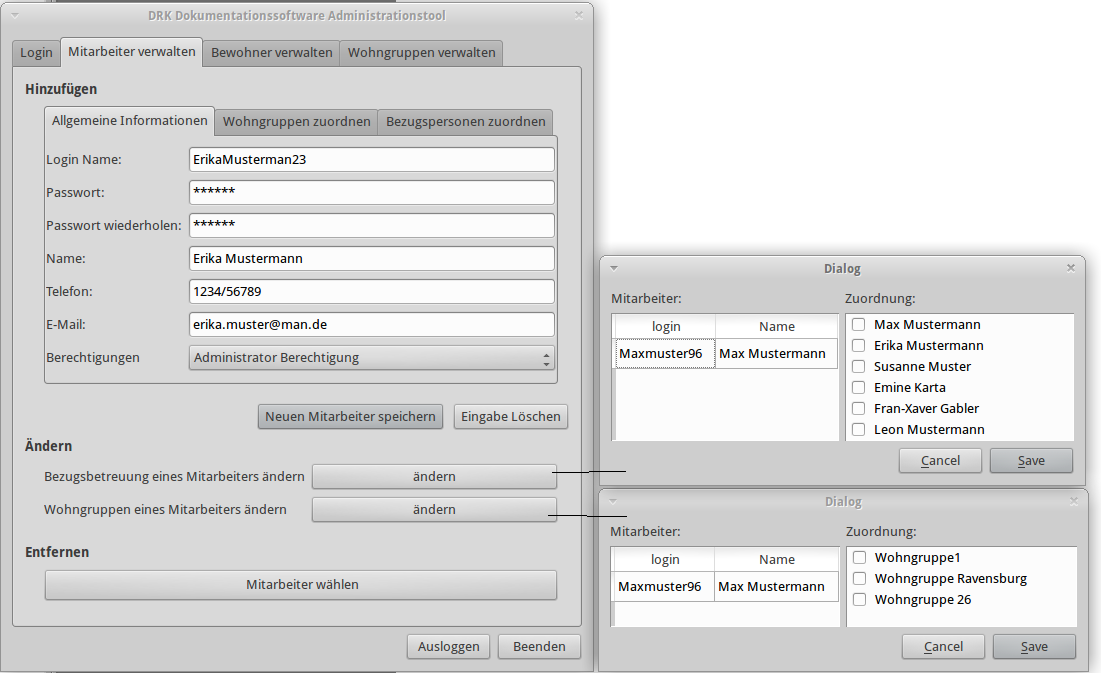
\includegraphics[keepaspectratio=true, width=0.85\textwidth]{pics/admin1.png}
		\caption{Mitarbeiter}
		\label{Admindialog Mitarbeiter}
	\end{center}
\end{figure*}
\FloatBarrier
\noindent
Mitarbeiter die keine Administratorenrechte haben können nur Informationen von Bewohner in ihrer Wohngruppe einsehen und nur von Bewohner deren Bezugsbetreuer sie sind verändern.
\newpage
\subsection{\EBP Client}
Der \EBP textit{Client} besitzt eine widgetbasierende GUI die aus folgenden Elementen besteht.
\begin{itemize}
	\item einer Menüleiste
	\begin{figure*}[h]
		\begin{center}
			
\includegraphics[keepaspectratio=true, width=0.55\textwidth]{pics/client_header.png}
			\caption{Menueleiste}
			\label{Menüleiste, fixiert an der oberen Seite des Programms}
		\end{center}
	\end{figure*}
	\FloatBarrier
	\noindent
	Hier wird der Inhalt des Hauptfensters gespeichert, die zusätzlichen Widgets aus-, bzw eingeblendet oder der Mitarbeiter ausgeloggt.
	\item einem Informationswidget
	\begin{figure*}[h]
		\begin{center}
			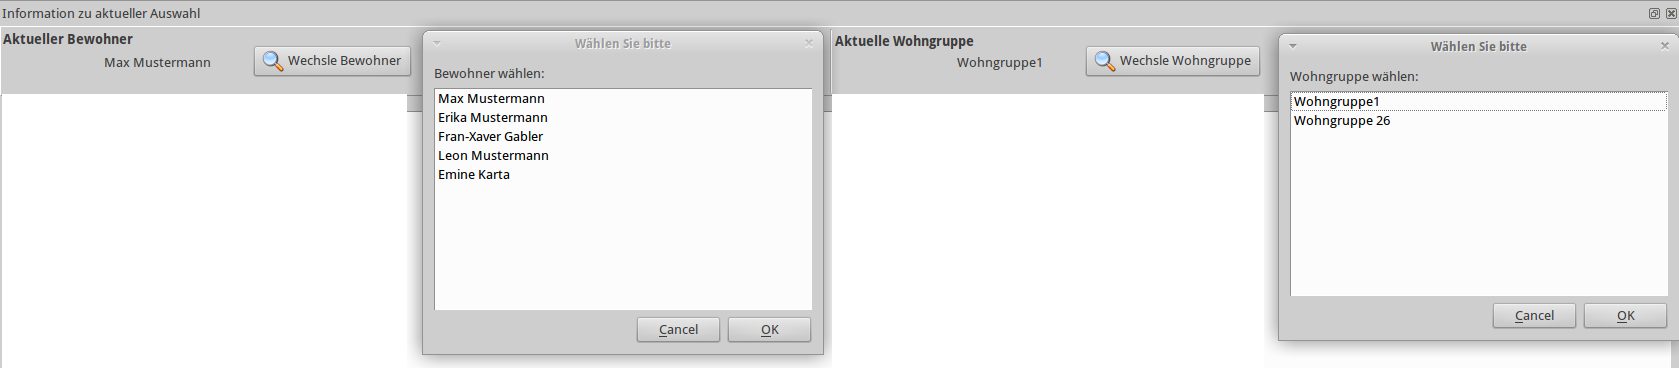
\includegraphics[keepaspectratio=true, width=0.95\textwidth]{pics/client_info.png}
			\caption{Informationswidget}
			\label{Bewohner- und Stationswidget}
		\end{center}
	\end{figure*}
	\FloatBarrier
	\noindent
	Hier der momentan ausgewählte Bewohner und dessen Station angezeigt, zum ändern öffnet sich bei Auswahl des jeweiligen Buttons ein Popup mit allen Stationen für die der Mitarbeiter berechtigt ist, bzw. alle Bewohner der jeweiligen Station.
	\newpage
	\item einem Navigationsmenü
	\begin{figure*}[h]
		\begin{center}
			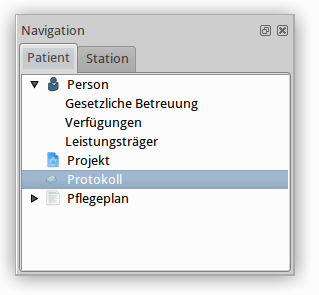
\includegraphics[keepaspectratio=true, width=0.35\textwidth]{pics/client_navi.png}
			\caption{Navigationswidget}
			\label{Navigationsmenü}
		\end{center}
	\end{figure*}
	\FloatBarrier
	\noindent
	Im Navigationsmenü wird der Inhalt des Hauptfensters ausgewählt.
	\item dem Mainwindow
	\begin{figure*}[h]
		\begin{center}
			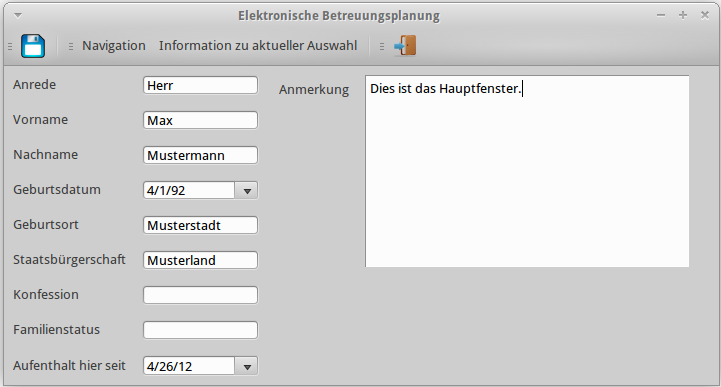
\includegraphics[keepaspectratio=true, width=0.95\textwidth]{pics/client_main.png}
			\caption{Mainwindow}
			\label{Hauptfenster}
		\end{center}
	\end{figure*}
	\FloatBarrier
	\noindent
	Das eigentliche Hauptfenster dient zur Ein-/Ausgabe von Daten und bezieht sich immer auf den im Informationswidget ausgewählten Bewohner, bzw die ausgewählte Wohngruppe. Um hier eingegebene Daten zu sichern muss der Speichern-Knopf in der Menüleiste betätigt werden.
\end{itemize}

\newpage
\subsection{Lokalisierung}
Sowohl der AdminDialog wie auch die \EBP sind komplett lokalisierbar. Qt stellt dafür einen einfachen Mechanismus zur Verfügung. Jeder zu lokalisierende String wird dabei von eimem Makro umschlossen. Das 
\subsection{Erstellen der Anwendung}
\subsubsection{Abhängigkeiten}
\paragraph{Zur Laufzeit:}
\begin{itemize}
	\item \textbf{odb} - ODB Laufzeitbibliothek
	\item \textbf{odb-mysql} - MySQL Backend für ODB
	\item \textbf{odb-qt} - QT integration für ODB
	\item \textbf{qt} - QT Framework
\end{itemize}
\paragraph{Zur Compilezeit:}
\begin{itemize}
	\item \textbf{CMake} - Buildsystem
	\item \textbf{ODB Toolchain} - Enthält den Precompiler
	\item \textbf{GCC} - GNU Compiler Collection
\end{itemize}
\subsubsection{Kompilieren der Quellen}
Die komplette Anwendung kann im Wurzelverzeichnis des Projekts gebaut werden:\\
\begin{lstlisting}
$ cmake .
\end{lstlisting}
Generiert das benötigte Makefile.\\
Ist dies erfolgreich abgeschlossen, wird mit\\
\begin{lstlisting}
$ make
\end{lstlisting}
der eignetliche Kompiliervorgang gestartet.\\
\subsubsection{Vorbereiten der Datenbank}
Um die Datenbank zu initialisieren befindet sich ein Shell-Script im EBPdb Verzeichnis:\\
\begin{lstlisting}
$ ./initDB.sh -u root -p "DATENBAKNAME"
\end{lstlisting}
